%
% CHAPTER: Entities, Represenations and Descriptions
%

\chapterimage{owl.pdf} % Chapter heading image

\chapter{Fundamental Elements}
\label{cha:Topics-and-Descriptions}

\begin{quote}
\begin{flushright}
\emph{We are all agreed that your theory is crazy. \\
The question which divides us is whether it is crazy enough.} \\
Niels Bohr
\end{flushright}
\end{quote}
\bigskip

The first step in quantifying our lack of knowledge involves the precise identification of the research entities of interest. The elements of this collection depend largely on the specific application of the theory of nescience. Each application requires a distinct set of entities, whether mathematical objects, living organisms, human needs, or otherwise. Fortunately, the process of quantifying what we do not know remains consistent across all such domains.

The next step is to devise a procedure for representing the identified entities as strings of symbols. Accurately encoding a research entity is a complex and unresolved epistemological challenge. The solution proposed within the theory of nescience is based on the concept of oracle Turing machine. The practical feasibility of this solution depends largely on the abstractness of the entities being studied. For example, encoding abstract mathematical objects poses significant difficulties and often requires an approximation. In contrast, encoding computer programs is relatively straightforward, as they are already expressed as strings.

Once a suitable method for encoding the original entities into string-based representations has been established, the final step is to produce a description. This description should be both accurate and concise, reflecting our current understanding of the representation. In the theory of nescience, descriptions are required to be computable, meaning that a computer must be able to fully reconstruct the original representation from its description. However, descriptions refer to representations, that is, the way entities are encoded, not to the entities themselves. As a result, how well a description captures knowledge about an entity depends largely on the quality of the representation used.

In this chapter, we will formalize these core concepts: entities, representations, and descriptions, among others. We will also explore what constitutes a perfect description, how to compute the combined representation of multiple entities, and how to describe a representation assuming some prior background knowledge. Additionally, we will examine the concept of a research area and its associated properties.

%
% Section: Entities
%

\section{Entities}
\label{sec:descriptions_entities}

Defining the nature of a research entity is a complex and unresolved philosophical problem. We approach this complexity from a fundamentally pragmatic perspective, rather than a philosophical-otological one. Our theory starts from the premise that there exists a non-empty set of \emph{entities}\index{Entities} that we seek to understand.

\begin{notation}
We represent the set of research entities of interest as $\mathcal{E}$.
\end{notation}

The contents of $\mathcal{E}$ depend on the specific domain in which theory of nescience is employed, and are usually aligned with a specific area of knowledge. Examples of entity sets could include: research components in mathematics (abstract); the kingdom Animalia (living entities); known and unknown human needs (abstract); all potential computer programs (strings), etc. From a formal point of view, $\mathcal{E}$ is not a well-defined set, since there is usually no rule or procedure for deciding which elements comprise this set.

The abstract nature of $\mathcal{E}$ offers certain advantages, but also imposes significant restrictions. The main restriction is that our definition of nescience is, in most cases, a non-computable quantity, which requires the use of approximations in practice. The main advantage is that the new concepts and methods presented in this book can be applied to a wide range of problems, not limited only to the search for new scientific knowledge.

In the theory of nescience, the possibility of using universal sets is excluded; that is, the existence of a set $\xi$ containing everything cannot be assumed. The problem with universal sets is that they contravene Cantor's theorem (see the example \ref{cantor_theorem}). Cantor's theorem proves that the power set $\mathcal{P}(\xi)$, consisting of all possible subsets of $\xi$, has more elements than the original set $\xi$. This contradicts the assumption that $\xi$ includes everything. In the theory of nescience, the set $\mathcal{E}$ must be a specific set.

\begin{example}[Cantor's theorem]\index{Cantor's theorem}
\label{cantor_theorem}
Cantor's theorem proves that for any set $A$, $d(A) < d\left(\mathcal{P}(A)\right)$. Consider $f: A \rightarrow \mathcal{P}(A)$, a function that maps each element $x \in A$ to the set $\{x\} \in \mathcal{P}(A)$; evidently, $f$ is injective, implying $d(A) \leq d\left(\mathcal{P}(A)\right)$. To substantiate that the inequality is strict, let's assume there exists a surjective function $g: A \rightarrow \mathcal{P}(A)$ and consider the set $B = \{ x \in A : x \notin g(x) \}$. As $g$ is surjective, there must exist a $y \in A$ such that $g(y) = B$. This, however, raises a contradiction, $y \in B \Leftrightarrow y \notin g(y) = B$. Consequently, the function $g$ cannot exist, therefore $d(A) < d\left(\mathcal{P}(A)\right)$.
\end{example}

In the theory of nescience, not all conceivable sets are acceptable, as some may give rise to paradoxes. Take, for example, Russell's paradox, which proposes a set $R$ consisting of all sets that are not members of themselves. The paradox arises when we try to discern whether $R$ is a member of itself (see the example \ref{ex:russell_paradox}). To avoid such problems, the theory of nescience is based on the Zermelo-Fraenkel axiom set, along with the Axiom of Choice. The \emph{axiom of separation}\index{Axiom of Separation} (if $P$ is a property with parameter $p$, then for any set $x$ and parameter $p$ there exists a set $y=\{u \in x : P(u) \}$ that includes all those sets $u \in x$ that have property $P$) allows the use of this notation only to construct sets that are subsets of already existing sets. A more extensive \emph{axiom of comprehension}\index{Axiom of comprehension} (if $P$ is a property, then there exists a set $y=\{u : P(u) \}$) would be required to allow sets like the one proposed by Russell's paradox. Russell's paradox arises from the use of an unrestricted comprehension principle. In the axioms of ZFC, and in the theory of nescience, the axiom of comprehension is considered false.

\begin{example}[Russell's Paradox]\index{Russell's Paradox}
\label{ex:russell_paradox}
Suppose $R$ is the set of all sets not members of themselves, such that $R = \{ x : x \notin x \}$. The contradiction arises when querying if $R$ is a member of itself. If $R$ is not a member of itself, by its own definition, it should be; conversely, if $R$ is declared to be a member of itself, its definition dictates it should not be. Symbolically, this can be written as $R \in R \Leftrightarrow R \notin R$.
\end{example}

In the theory of nescience, we do not address the classic problems of ontology, that is, the classification of entities that exist in the world and can be known. Furthermore, we do not attempt to resolve epistemological questions, such as how scientific knowledge is validated by evidence, or what the nature of that evidence is.

Once a set $\mathcal{E}$ of entities has been selected, the next step is to uniquely encode them as strings of symbols, which will make them easier to describe. A method for doing this encoding efficiently is described in the following section.

%
% Section: Representations
%

\section{Representations}
\label{sec:representations}

The representation of the entities that compose the set $\mathcal{E}$, which can be abstract in nature, poses important epistemological challenges that have been the subject of research for more than two millennia (see Section \ref{sec:scientific_representation} for a brief overview of the solutions proposed by the scientific community and their limitations). This book describes a possible solution to this complex problem, which has certain advantages, but also disadvantages. Our approach proposes dividing the problem of scientific representation into two interconnected subproblems: the encoding of entities by means of representations, and the modeling of these representations by means of descriptions. Thus, scientific models would explain the entities indirectly through their representations (see Figure \ref{fig:representationProblem} in the Introduction of the book, reproduced in this section for ease of reference). In this section we will focus on the aspects related to encoding, and in Section \ref{sec:descriptions_models} on the descriptions.

% A4
% \begin{figure}[t]
% \centering
% \begin{tikzpicture}
%     \node[draw, ellipse, minimum width=3cm] (entities) at (0,0) {Entities};
%     \node[draw, ellipse, minimum width=3cm] (representations) at (5,0) {Representations};
%     \node[draw, ellipse, minimum width=3cm] (descriptions) at (10,0) {Descriptions};
% 
%     \draw[-{Latex[length=3mm]}] (representations) -- node[above,midway] {encode} (entities);
%     \draw[-{Latex[length=3mm]}] (descriptions) -- node[above,midway] {model} (representations);
%     \draw[dashed,-{Latex[length=3mm]}] (descriptions) to [bend right=45] node[above,midway] {explain?} (entities);
% \end{tikzpicture}
% \caption{\label{fig:representationProblem}The Problem of Understanding}
% \end{figure}

% Octavo
\begin{figure}[t]
\centering
\begin{tikzpicture}
    \node[draw, ellipse, minimum width=1.5cm] (entities) at (0,0) {Entities};
    \node[draw, ellipse, minimum width=1.5cm] (representations) at (4.25,0) {Representations};
    \node[draw, ellipse, minimum width=1.5cm] (descriptions) at (9,0) {Descriptions};

    \draw[-{Latex[length=3mm]}] (representations) -- node[above,midway] {encode} (entities);
    \draw[-{Latex[length=3mm]}] (descriptions) -- node[above,midway] {model} (representations);
    \draw[dashed,-{Latex[length=3mm]}] (descriptions) to [bend right=45] node[above,midway] {explain?} (entities);
\end{tikzpicture}
\caption{\label{fig:representationProblem}The Problem of Understanding}
\end{figure}

Within the field of Kolmogorov complexity\index{Kolmogorov complexity}, the representation issue is tackled by presupposing that the set $\mathcal{E}$ is well-defined, countable, and that a total encoding function $f:\mathcal{E} \rightarrow \mathbb{N}$ exists, mapping the set of entities to the set of natural numbers (akin to Gödel numbering\index{Gödel numbering}). The nescience theory similarly embraces this concept of encoding entities via numbers, or, in other words, strings of symbols. However, our approach to the problem of encoding an arbitrary set $\mathcal{E}$ involves an inversion of the problem. This involves defining a partial function $\mathcal{O}_\mathcal{E}:\mathcal{S}^\ast \rightarrow \mathcal{E}$ that maps the well-defined set $\mathcal{S}^\ast$ (comprising all possible finite strings from an alphabet $\mathcal{S}$) to the potentially non-countable and non-well defined set $\mathcal{E}$ containing the entities of interest.

Our function $\mathcal{O}_\mathcal{E}$, which depends on the set $\mathcal{E}$, operates much like an oracle (taking inspiration from the concept of an oracle Turing machine\index{Oracle Turing machine} as per Definition \ref{def:Oracle-Turing-Machine}). This function has the capacity to entirely reconstruct an entity $\mathcal{O}_\mathcal{E} (x) \in \mathcal{E}$ using its encoding string $x \in \mathcal{S}^\ast$, without the need for additional information. Evidently, this oracle is an abstract concept, and its construction in the real world would be impossible for most sets $\mathcal{E}$. However, the theoretical existence of this oracle assists in the elucidation and verification of key attributes of the scientific discovery process. Due to its oracle nature, $\mathcal{O}_\mathcal{E}$ has limitations with respect to the mathematical operations in which it can be used, as will be explained in the subsequent paragraphs.

Our premise is based on the assumption that there exists a single, objective physical world that is independent of observers. In addition, we assume that, for certain collections of entities $\mathcal{E}$, it is logically coherent to postulate the existence of an oracle $\mathcal{O}_\mathcal{E}$ (see the discussion of the scientific representation problem in Section~\ref{sec:scientific_representation}).

For the purposes of this book, without any loss of generality, we will exclusively regard binary strings as the means of encoding entities.

\begin{definition}
\label{def:descriptions_topic}
Given $\mathcal{E}$ as a set of entities, a \emph{representation function}\index{Representation function} is defined as an oracle partial function $\mathcal{O}_\mathcal{E}:\mathcal{B}^\ast \rightarrow \mathcal{E}$ that maps elements of the set $\mathcal{B}^\ast$, which comprises all conceivable finite binary strings, to the elements of the set $\mathcal{E}$, corresponding to the entities under examination.
\end{definition}

Within this framework, only the elements of the set $\mathcal{B}^\ast$, that is, binary strings, are eligible to serve as representations of entities (see problem of ontology\index{Problem of ontology} in Section \ref{sec:scientific_representation}). We do not permit other forms of physical models, including drawings, unless they can be transcribed into binary strings. We do not distinguish between scientific representations and other forms of representations (see representational demarcation\index{Representational demarcation} in Section \ref{sec:scientific_representation}). The oracle assumes the responsibility of determining which entity is encoded by each representation. It is also pivotal to note that the oracle $\mathcal{O}_\mathcal{E}$ is a partial function, meaning not all potential strings represent entities (targetless models\index{Targetless models} are allowed in the theory of nescience, see Section \ref{sec:targetless_representations} and Section \ref{sec:scientific_representation}).

\begin{example}
\label{ex:not_unique_oracle}
For a given set of entities $\mathcal{E}$, the existence of a representation oracle $\mathcal{O}_\mathcal{E}$ does not imply its uniqueness. For instance, a binary negation oracle (which transforms the zeros of a binary string into ones, and the ones into zeros), assigning to each string $x \in \mathcal{B}^\ast$ the entity $\mathcal{O}_\mathcal{E} \left( \neg x \right)$, would also qualify as a representation function.
\end{example}

Rather than deploying individual oracles, we could have employed a universal oracle machine. This is a machine $\mathcal{U}_\mathcal{O}$ which, given the encoding of an oracle $\mathcal{O}_\mathcal{E}$ and a string $s$ as input, computes $\mathcal{U}_\mathcal{O} \left( \langle \mathcal{O}_\mathcal{E}, s \rangle \right) = \mathcal{O}_\mathcal{E} \left( s \right)$. Universal machines are particularly applicable to the universal set $\xi$, encompassing all entities. However, such an approach would complicate the process of scientific discovery in practical terms. Instead, we choose to work with entity sets $\mathcal{E}$ corresponding to different areas of knowledge, choosing a single oracle $\mathcal{O}_\mathcal{E}$ for each set $\mathcal{E}$ (the most suitable one according to our current knowledge and our practical needs).

\begin{example}
\label{ex:description_dna}
Consider the case when the subjects of study are animals. Initially, one might use detailed physical descriptions of the animals as encodings. In this scenario, the oracle would be a hypothetical machine capable of reconstructing the original animal from its description. As our understanding of biology advances, we might instead adopt an alternative encoding based on the animals' DNA. Both of these encodings serve as valid representations of the entities.
\end{example}

As illustrated in Example \ref{ex:not_unique_oracle} and Example \ref{ex:description_dna}, the entities in $\mathcal{E}$ can be encoded in multiple ways (see the problem of style\index{Problem of style} in Section \ref{sec:scientific_representation}). Different oracles accommodate different encoding schemes. Some strings provide more accurate representations of an entity than others (see the standard of accuracy\index{Standard of Accuracy} in Section \ref{sec:scientific_representation}). The optimal representation depends on the type of questions we aim to answer. Using a particular encoding style with an oracle designed for a different style may lead to unexpected outcomes. Our objective should be to employ representations that minimize the size of the oracle—that is, the amount of prior knowledge presumed to be embedded within it.

\begin{example}
Consider $\mathbf{X}_t$ as a time series consisting of $m$ measurements $x_1, \ldots, x_m$ collected at fixed intervals from a physical phenomenon exhibiting sinusoidal behavior. Suppose we have trained a multi-layer perceptron\index{Multi-layer perceptron} neural network $nn$ that perfectly fits the data, meaning it returns $x_t$ when given a time $t$ as input. By analyzing the cycles in the time series, one would naturally identify a sine function as the most appropriate model for the underlying physical process. However, no existing machine learning methodology would arrive at this conclusion if provided solely with the neural network's architecture (i.e., the number of layers, their sizes, and the trained weights). Clearly, the oracle is sufficiently powerful to recognize this underlying structure.
\end{example}

Remember that the oracle operates as a partial function, meaning that not every string must represent an entity. The less information a representation contains, the more difficult it becomes to understand how the oracle works. It is essential to be cautious with representations that fail to capture the full structure of the original entities, as this can introduce bias into our analyses. Chapter \ref{chap:Miscoding} offers a detailed discussion of the types of errors arising from the miscoding of abstract entities, emphasizing that representations must not only correspond to entities, but also that entities must be relevant to their representations (see the requirement of directionality\index{Requirement of directionality} in Section \ref{sec:scientific_representation}).

We employ an oracle function rather than an oracle relation $\mathcal{R}_\mathcal{O} \subset \mathcal{B}^\ast \times \mathcal{E}$, not to merely associate strings with their corresponding entities, but to reconstruct an entity from its representation. The oracle's ability to recover original entities underpins our capacity to make hypotheses about entities based on their representations (see surrogative reasoning\index{Surrogative reasoning} in Section \ref{sec:scientific_representation}). According to the theory of nescience, scientific inquiry involves not only learning how to encode entities properly but also understanding the mechanisms by which oracles decode them. For scientific inquiry to be practically effective, these oracles should ideally be minimal in size.

The purpose of encoding entities in the theory of nescience differs fundamentally from that in Shannon's information theory (see Chapter \ref{chap:Coding}), as illustrated in Example \ref{ex:shannon_encoding}.

\begin{example}
\label{ex:shannon_encoding}
Take, for instance, a set $\mathcal{E}$ consisting of two books: "The Ingenious Nobleman Sir Quixote of La Mancha" and "The Tragedy of Romeo and Juliet". We might encode the first book with the string "0" and the second with the string "1". While these strings allow us to uniquely identify each book within the set, they do not qualify as valid encodings within the framework of the theory of nescience. In information theory, the goal is to uniquely identify an object based on a reference, assuming mutual agreement between the sender and the receiver about the mapping from references to objects. In contrast, the theory of nescience seeks representations that preserve the richness and detail of the original entities. For example, it would be impossible to hypothesize about Cervantes' influence on Shakespeare using only the strings "0" and "1".
\end{example}

One possible response to the limitation discussed in Example \ref{ex:shannon_encoding}, where entities are encoded using overly simplistic strings that fail to capture their internal structure, would be to require the set $\mathcal{E}$ to be infinite, as is done in Kolmogorov complexity. This requirement avoids pathological cases in which too many entities are assigned trivial or arbitrary encodings. However, merely increasing the size of $\mathcal{E}$ does not solve the fundamental issue: even with an infinite set of entities, many encoding schemes still fall short of supporting surrogative reasoning. That is, they do not allow us to make meaningful inferences about the original entities based solely on their representations. To enable such reasoning, the encoding must preserve essential structural and semantic features of the entities, not just their identity.

We distinguish between \emph{knowable} and \emph{unknowable} entities. Knowable entities are those that can, in principle, be understood through scientific inquiry (see Section \ref{sec:what-is-an-entity}). Unknowable entities, on the other hand, lie beyond the reach of human comprehension—either because they are inherently inaccessible to observation and reasoning, or because they exceed the cognitive or methodological limits of science.

\begin{definition}
We say that an entity $e \in \mathcal{E}$ is \emph{knowable}\index{Knowable entity} if there exists at least one $r \in \mathcal{B}^\ast$ such that $\mathcal{O}_\mathcal{E}(r) = e$. An entity $e \in \mathcal{E}$ is \emph{unknowable}\index{Unknowable entity} if it is not knowable.
\end{definition}

A priori, it is not possible to determine whether an entity $e \in \mathcal{E}$ is knowable, unknowable, or only partially knowable. Identifying suitable knowable entities for study is a matter of trial and error. In this book, we say nothing further about unknowable entities, except to note that their unknowability can neither be proven nor discovered.

\begin{definition}
Let $e \in \mathcal{E}$ be a knowable entity. We define the \emph{set of representations}\index{Set of representations} for $e$, denoted by $\mathcal{R}_e$, as $\{ r \in \mathcal{B}^\ast : \mathcal{O}_\mathcal{E} (r) = e \}$.
\end{definition}

In Figure \ref{fig:entities_topics_1}, we present a depiction of a hypothetical oracle mapping from the set of finite binary strings $\mathcal{B}^\ast$ to the set of entities $\mathcal{E}$. The figure also highlights a particular entity $e_1$, the subset of strings $\mathcal{R}_{e_1}$ that represent this entity, and a specific representation $r_1$. Since the set $\mathcal{E}$ is, in general, not well defined, the inverse function $\mathcal{O}_\mathcal{E}^{-1}(e_1)$ cannot be computed in practice.

\begin{figure}[t]
\centering
\begin{tikzpicture}[line width=1pt, >=Stealth]

%--- left outer ellipse -------------------------------------------
\draw[fill=gray!25] (-3,0) ellipse (1.5 and 2);          % 𝔅* (grey background)
\node at (-4.2,-2.4) {$\mathcal{B}^{*}$};

%--- left inner region R_{e1} -------------------------------------
\draw (-3,1) ellipse (1 and 0.7);                      % 𝑅_{e1}
\node[anchor=east] at (-2.8,1) {$r_{1}$};
\fill (-2.7,1) circle (5pt);                           % black dot r1
\node at (-3.2,0) {$\mathcal{R}_{e_1}$};

%--- right outer ellipse ------------------------------------------
\draw (3,0) ellipse (1.5 and 2);                         % ℰ (white background)
\node at (4.4,-2.4) {$\mathcal{E}$};

%--- right inner grey region --------------------------------------
\draw[fill=gray!25] (3,0.25) ellipse (1.3 and 1.5);

%--- entities e1 and e2 -------------------------------------------
\fill (3.1,1.3) circle (5pt);                          % e1 dot
\node[anchor=west] at (3.3,1.3) {$e_{1}$};

\fill (3.2,-1.5) circle (5pt);                         % e2 dot
\node[anchor=west] at (3.4,-1.5) {$e_{2}$};

%--- oracle barrier -----------------------------------------------
\draw (0,-2.4) -- (0,2.4);
\node[below=2pt] at (0,-2.4) {oracle};

%--- curved two-piece arrow (solid then dashed) -------------------
\path
  (-2.2,1)                                     % start at r1
  .. controls (-1,2.2) and (-0.4,2) .. (0,2)   % solid part up to barrier
  node[pos=0.55]{};                            % (dummy to split the path)

\draw[line width=1pt] (-2.7,1) .. controls (-1.5,2) and (-0.4,2) .. (0,2);

\draw[line width=1pt,dashed,-Stealth]
      (0,2) .. controls (1.3,2.1) and (2.4,1.9) .. (3.05,1.3);

\end{tikzpicture}
\caption{\label{fig:entities_topics_1}Encodings and Entities}
\end{figure}

% \begin{figure}[h]
% \centering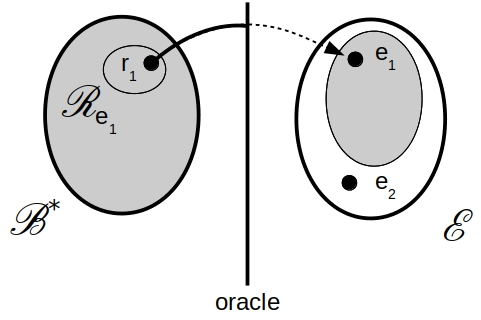
\includegraphics[scale=0.5]{entities_topics_1}
% \caption{\label{fig:entities_topics_1}Encodings and Entities.}
% \end{figure}

A consequence of working with finite strings as representations is that some entities may not be encoded by any representation (see the gray areas in Figure \ref{fig:entities_topics_1}; in particular, the entity $e_2$ is not encoded by any string). Intuitively, this reflects the fact that, in certain domains of knowledge, the number of possible problems far exceeds the number of available solutions.

\begin{example}
If the collection of entities under study consists of real numbers, then there exist numbers that cannot be encoded using finite binary strings. This is because the set $\mathbb{R}$ has the cardinality of the continuum, whereas the set $\mathcal{B}^\ast$ is countable.
\end{example}

Since our knowledge of the entities and the internal workings of the oracle is incomplete, in practice we work with a different set of strings, denoted by $\hat{\mathcal{R}}_e$, which we believe are close approximations of the true representations $\mathcal{R}_e$ that encode the entity $e$. The elements of this set typically change over time, as our understanding of the entities in $\mathcal{E}$ and of how the oracle encodes them improves. The more abstract the set of entities is, the more difficult it becomes to approximate them as strings (see Chapter \ref{chap:Miscoding}).

\begin{example}
\label{ex:luminiferous_ether}
The entity "luminiferous ether"\index{Luminiferous ether} was a theoretical postulate describing a hypothetical medium through which light was believed to propagate. It was proposed to explain how wave-based light could travel through empty space. However, in 1887, the Michelson-Morley experiment\index{Michelson-Morley experiment} provided strong evidence against the existence of ether. Later, Einstein's special theory of relativity\index{Theory of relativity} offered a successful explanation for the propagation of light in a vacuum, leading to the complete abandonment of the ether concept.
\end{example}

If the chosen oracle is not minimal, determining whether a string is a valid representation of an entity requires understanding the internal workings of the oracle. A *non-minimal oracle* is one in which part of the information needed to reconstruct the original entity is embedded within the oracle itself, rather than being explicitly encoded in the representation string. Although using non-minimal oracles can simplify the research process by offloading complexity to the oracle, it obscures the boundary between what is encoded and what is assumed, making it harder to analyze or generalize the representation mechanism.

\begin{remark}
One of the fundamental challenges in science—and in human intellectual activity more broadly—is the tendency to confuse symbols with the things they represent. The theory of nescience has been carefully designed to avoid this issue by clearly distinguishing between research entities and their representations. However, making this distinction explicit at every step would render the book unnecessarily difficult to read. We have aimed to strike a balance between clarity of exposition and rigor of definition. Occasionally, especially when introducing new ideas, we use the term \emph{topic} to refer broadly to an entity, a representation, or both. Nevertheless, in all mathematical definitions and propositions, this distinction is made unambiguous. In case of any uncertainty, the formal definitions should be taken as the definitive reference.
\end{remark}

%
% Section: Invalid Representations
%
\section{Invalid Representations}
\label{sec:invalid_representations}

It may happen that the representation we are using for an entity $e \in \mathcal{E}$ is incorrect. That is, instead of working with a string $r \in \mathcal{B}^\ast$ that perfectly encodes $e$, we are studying another string $r' \in \mathcal{B}^\ast$ which is, hopefully, close to $r$ but not necessarily identical. We are interested in computing the distance between the string $r'$ and the correct representation $r$ as a quantitative measure of the error introduced by using an incorrect encoding (see Chapter \ref{chap:Miscoding}). Unfortunately, we do not know $r$, since in most practical applications there does not exist a computable function from $\mathcal{E}$ to $\mathcal{B}^\ast$. The only tool at our disposal is an abstract oracle machine $\mathcal{O}_\mathcal{E}$ that knows which strings represent each entity. Recall from Section \ref{sec:representations} that we propose to address the scientific representation problem by introducing an abstract oracle $\mathcal{O}_\mathcal{E} : \mathcal{B}^\ast \rightarrow \mathcal{E}$, which maps the set $\mathcal{B}^\ast$ of all finite binary strings to the set $\mathcal{E}$ of entities under study.

We begin by distinguishing between valid representations, strings that contain all the information required by the selected oracle to reconstruct an entity, and non-valid representations.

\begin{definition}
Let $\mathcal{E}$ be a collection of entities, and let $\mathcal{O}_\mathcal{E}$ be a decoding function. We define the set of \emph{valid}\index{Valid Representation} representations for $\mathcal{E}$ with respect to the encoding function $\mathcal{O}_\mathcal{E}$, denoted by $\mathcal{R}^\star_{\mathcal{O}_\mathcal{E}}$, as the subset of representations that perfectly encode an entity in $\mathcal{E}$, according to $\mathcal{O}_\mathcal{E}$.
\end{definition}

The set $\mathcal{R}^\star_{\mathcal{O}_\mathcal{E}}$ is generally unknown, as it is a subset of $\mathcal{B}^\ast$ whose definition depends on an abstract and not well-defined oracle. Intuitively, a representation is considered valid if it contains all the necessary information for the oracle to reconstruct the original entity without relying on any external sources. A valid representation must not include incorrect symbols, nor omit any relevant information, otherwise, the oracle would be unable to reconstruct the entity accurately.

Furthermore, we require that the oracle can not only reconstruct an entity from a representation, but also derive the set of valid representations for a given entity. From this perspective, a representation that includes non-relevant information cannot be considered valid, since that extraneous part cannot be generated by the oracle solely from the entity.

\begin{example}
The astronomical data used during the time of Ptolemy to record the positions of celestial bodies throughout the year constituted a non-valid encoding of the entity "position of celestial bodies," due to its inaccuracy. A better encoding was later provided by the more precise observations of Tycho Brahe. Today, we possess even more accurate encodings. Adding the name of the person who collected the data to the dataset would be an example of a representation that includes non-relevant information.
\end{example}

Recall that, in our framework, we only allow representations of entities in the form of finite binary strings. Drawings, mathematical formulas, or datasets may serve as representations, provided they can be encoded as binary strings and are recognized as valid by the selected oracle. Each string represents one, and only one, entity. Naturally, different oracles may define different sets of valid representations. Throughout this work, we assume that a specific representation oracle $\mathcal{O}_\mathcal{E}$ has been chosen to encode the set $\mathcal{E}$ of entities under study.

\begin{notation}
We will denote the set of valid representations of $\mathcal{E}$ by $\mathcal{R}^\star_\mathcal{E}$ when there is no ambiguity regarding the oracle $\mathcal{O}_\mathcal{E}$ in use.
\end{notation}

We can similarly define the set of valid representations for an individual entity $e$.

\begin{definition}
We define the set of valid representations for an entity $e \in \mathcal{E}$, denoted by $\mathcal{R}^\star_e$, as the subset of representations that perfectly encode the entity $e$; that is, $\mathcal{R}^\star_e = \mathcal{R}^\star_\mathcal{E} \cap \mathcal{R}_e$.
\end{definition}

As we have seen in Example \ref{ex:description_dna} there could be more than one valid representation for some entities, even it the oracle is restricted to a particular style. It might also happen that the set of valid representations is empty, that is, there is no valid representation for that entity. In that case the entity will be unknowable.

\begin{notation}
We denoted by $r^\star_e \in \mathcal{R}^\star_\mathcal{E}$ the fact that $r$ is a valid representation of the entity $e$.
\end{notation}

A consequence of working with approximations instead of true representations is that some of the candidate strings currently in use may encode a different entity than the one we intended to study.

\begin{example}
\label{ex:polywater}
In 1961, Soviet physicist Nikolai Fedyakin conducted a series of experiments that appeared to reveal a new form of water. This substance, named polywater\index{Polywater}, exhibited unusual properties: a higher boiling point, a lower freezing point, and much greater viscosity than ordinary water. However, later experiments demonstrated that polywater was simply ordinary water contaminated with small amounts of impurities.
\end{example}

We can safely assume (without logical contradiction) that the oracle machine not only knows which representations correspond to which entities, but also how far any string $r \in \mathcal{B}^\ast$ is from being a valid representation $r^\star_e \in \mathcal{R}^\star_\mathcal{E}$.

If a representation $r$ is non-valid, the oracle will identify the closest valid representation and assume they both refer to the same entity.

The oracle defines an equivalence relation that partitions the set $\mathcal{B}^\ast$ into equivalence classes. Each class corresponds to an entity in $\mathcal{E}$, although it may happen that some entities in $\mathcal{E}$ do not have any associated class, these are what we call the unknowable unknowns\index{Unknowable unknown}. Every string is associated with some entity, but some representations are better than others (i.e., they yield lower nescience). No string can belong to more than one entity. Moreover, for any given collection $\mathcal{E}$, multiple valid oracles may exist.

\begin{definition}
Let $\mathcal{B}^\ast / \mathcal{O}$ be the quotient set defined by the oracle's equivalence relation over the set of binary strings. We call each class in this quotient set an \emph{entity class}\index{Entity class}, denoted by $[e]$, that is, $[e] \in \mathcal{B}^\ast / \mathcal{O}$.
\end{definition}

%
% Section: Joint Representations
%

\section{Joint Representations}
\label{sec:descriptions_joint_topic}

We saw in the previous section that there is more than one way to encode an entity $e \in \mathcal{E}$, this collection of encodings is what we called the set $\mathcal{R}_e$ of representations of the entity. Some of these representations are of high quality, in the sense that they contain all the information required by the oracle to reconstruct (by whatever means the oracle employs) the original entity. However, the set $\mathcal{R}_e$ also includes low-quality representations, that is, representations that lack many of the details necessary to fully reconstruct the entity. Moreover, $\mathcal{R}_e$ may contain representations that include incorrect information: symbols that the oracle will automatically disregard during reconstruction but that may mislead us when trying to understand the entity.

If we want to increase our knowledge about an entity, we must identify the best possible representation for that entity, that is, one that is both complete and correct. One way to achieve this is to try different strings until we discover a high-quality representation. However, this method can be extremely time-consuming and impractical. A more efficient approach is to enhance a poor representation by adding missing symbols or by combining known representations that each contain partial information. Both approaches require introducing the concept of a joint representation.

\begin{definition}
Let $s, t \in \mathcal{R}_\mathcal{E}$ be two different representations. The \emph{joint representation}\index{Joint Representation} of $s$ and $t$ is defined as the concatenated string $st$.
\end{definition}

\begin{example}
\label{ex:lung_cancer}
Suppose the research entity $e$ of interest is the set of causes of lung cancer. To study this entity, we have measured a collection of risk factors in a random sample of the population (smoking, exercise, diet, age, etc.). However, due to a flaw in the sampling procedure, all the samples correspond to a specific subgroup of the population, for instance, males. This dataset constitutes a representation $s$ of our entity $e$, but a poor one, as it is strongly biased. If we have a second representation $t$, corresponding to sample data from females, the joint representation $st$ will be superior to either $s$ or $t$ considered in isolation.
\end{example}

It would be desirable for the set of representations $\mathcal{R}_\mathcal{E}$ to be closed under the operation of concatenation, meaning that if $s$ and $t$ are representations of an entity $e$, then their concatenation $st$ would also be a representation of some entity (not necessarily the same one). Unfortunately, this is not the case, since the oracle function is partial; it does not assign an entity to every possible binary string. Moreover, we do not even require the set of representations $\mathcal{R}_e$ for a given entity $e$ to be closed under concatenation. It is entirely possible that two strings $s \in \mathcal{R}_e$ and $t \in \mathcal{R}_e$ produce a concatenated string $st$ that does not belong to $\mathcal{R}_e$.

The concept of joint representation is defined for any pair of strings $s, t \in \mathcal{R}_\mathcal{E}$, even if they do not belong to the same set of representations $\mathcal{R}_e$, that is, even when $\mathcal{O}_\mathcal{E}(s) \neq \mathcal{O}_\mathcal{E}(t)$. This ability to combine representations of different entities will prove particularly useful for the discovery of new research entities that are currently unknown (see Section \ref{sec:New_Research_Topics}).

The operation of string concatenation is associative; that is, for all $r, s, t \in \mathcal{R}_\mathcal{E}$, we have $(rs)t = r(st)$. This property underlies the algebraic structure of the set of representations.

\begin{proposition}
The set $\mathcal{R}_\mathcal{E}$ of representations, together with the operation of concatenation, has the structure of a free monoid.
\end{proposition}
\begin{proof}
As shown in Section \ref{sec:strings}, the operation of string concatenation on $\mathcal{R}_\mathcal{E}$ is associative, and the empty string $\lambda$ serves as the identity element.
\end{proof}

We do not require the operation of joining representations to be commutative with respect to the oracle function. Given representations $s, t \in \mathcal{R}_\mathcal{E}$, it may happen that the concatenated strings $st$ and $ts$ represent different entities—that is, $\mathcal{O}_\mathcal{E} \left( st \right) \neq \mathcal{O}_\mathcal{E} \left( ts \right)$.

The concept of joint representation can be extended to any arbitrary, but finite, collection of representations. This allows us to incorporate multiple partial representations into our research or to use them in the process of discovering new entities.

\begin{definition}
Let $r_1, r_2, \ldots, r_n \in \mathcal{R}_\mathcal{E}$ be a finite collection of representations. The \emph{joint representation} of $r_1, r_2, \ldots, r_n$ is defined as the concatenated string $r_1 r_2 \ldots r_n$.
\end{definition}

Unfortunately, the set $\mathcal{R}_\mathcal{E}$ is not closed under the operation of concatenation of multiple, finite, representations.

We have seen that the concatenation of two or more representations of an entity can result in a string that encodes a different entity from the original. Remarkably, this phenomenon can occur even when the individual representations being concatenated all correspond to the same entity. This non-trivial behavior opens the door to a novel strategy for scientific discovery: the generation of new, previously unknown entities through the systematic combination of representations of known entities.

\begin{example}
Consider a research scenario in which the entities under study are chemical compounds, and the representations are strings encoding molecular descriptors. Suppose $s$ encodes a compound known for its anti-inflammatory properties, and $t$ encodes a structurally similar compound with anti-viral properties. While both $s$ and $t$ individually map to well-known compounds via the oracle, the concatenation $st$ may correspond to a novel hybrid molecule whose biological activity has not yet been characterized. In this case, $st$ represents a new research entity, possibly a candidate for drug discovery—that was not explicitly part of the original knowledge base.
\end{example}

%
% Section: Descriptions
%

\section{Descriptions}
\label{sec:descriptions_models}

So far, our goal in working with strings from $\mathcal{B}^\ast$ has been to construct encodings, or representations, that are as complete and detailed as possible for the entities in $\mathcal{E}$, regardless of their length. However, as stated in the preface of this book, human understanding requires the formulation of concise models of these entities, since human reasoning cannot operate effectively on lengthy representations.

\begin{example}
In Example \ref{ex:lung_cancer}, we showed that a good representation of the entity "lung cancer" could be a dataset in which various risk factors are measured. However, smokers do not decide to quit smoking because they have studied and understood this extensive dataset. Rather, they do so because they understand the much simpler derived model: "smoking increases the risk of lung cancer."
\end{example}

A description or model\footnote{In the theory of nescience, the terms "description" and "model" are used interchangeably.} is a finite binary string that is mapped to a representation of an entity (see Figure \ref{fig:entities_topics_models} in Chapter \ref{chap:Introduction}). Importantly, descriptions do not directly model the entities themselves (i.e., the target systems); instead, they operate on representations of those entities (encodings in the form of strings) serving as approximations of the original entities through those representations.

In the theory of nescience, we require that descriptions be computable, so that the original representations can be fully and effectively reconstructed from them. This requirement of computability allows us to clearly define the limits of the concept of a "description." For example, paradoxes involving self-reference, such as the Berry paradox\index{Berry paradox} (i.e., "the smallest positive integer not definable in less than twelve words," see Chapter \ref{chap:Introduction}), can be addressed within the framework of computability.

\begin{definition} [Model]
\label{def:description_model}
Let $d \in \mathcal{B}^\ast$ be a binary string of the form $d = \langle TM, a \rangle$, where $TM$ is the encoding of a prefix-free Turing machine and $a$ is the input string to that machine. If $TM(a)$ is defined, then $d$ is called a \emph{description}\index{Description}.
\end{definition}

Intuitively, a description consists of two parts: a Turing machine that captures and compresses the regularities present in the representation, and a string that contains what remains, that is, the incompressible or random part.

\begin{definition}
\label{def:descriptions_model}
We define the \emph{set of descriptions}\index{Set of descriptions}, denoted by $\mathcal{D}$, as:
\[
\mathcal{D} = \{ d \in \mathcal{B}^\ast : d = \langle TM,a \rangle \wedge TM(a) \downarrow \}.
\]
Let $r \in \mathcal{B}^\ast$ be a representation. We define the set of \emph{descriptions for $r$}, denoted by $\mathcal{D}_r$, as:
\[
\mathcal{D}_r = \{ d \in \mathcal{D} : TM(a) = r \}.
\]
Finally, given an entity $e \in \mathcal{E}$, we define the set of \emph{descriptions for $e$}, denoted by $\mathcal{D}_e$, as:
\[
\mathcal{D}_e = \{ d \in \mathcal{D} : \exists r \in \mathcal{R}_e,\, TM(a) = r \}.
\]
\end{definition}

From an ontological point of view, descriptions are string-based representations that satisfy the additional requirement of being computable. In this sense, descriptions are a subset of representations, and thus, there can exist descriptions that describe other descriptions. However, in practice, it is not advisable to use descriptions as representations of entities, since what we seek in a good representation is the inclusion of as many details as possible about the original entities, not a concise encoding. Using descriptions in place of representations would make the task of scientific discovery considerably more difficult for humans.

Since each description corresponds to one, and only one, representation, we can define a function that maps descriptions to representations. Given that descriptions are encoded Turing machines, it is natural to define this mapping using a universal Turing machine. As a result, not only are individual descriptions of representations computable, but the function that maps descriptions to representations is also computable.

\begin{definition}
We call \emph{description function}\index{Description function}, denoted by $\delta$, any universal Turing machine $\delta : \mathcal{D} \rightarrow \mathcal{B}^\ast$ that maps descriptions to their corresponding representations.
\end{definition}

If $d = \langle TM, a \rangle$ is a description of the representation $r$, then we have that $\delta \left( d \right) = \delta \left( \langle TM, a \rangle \right) = TM(a) = r$.

Inspired by the Occam's razor principle\index{Occam's razor principle}\footnote{The Occam's razor principle refers to the number of assumptions in an explanation, not to the length of the explanation itself.}, if two explanations are equivalent, we should prefer the shorter one. Accordingly, the limit of what can be known, or understood, about a representation, that is, its perfect model, is given by the shortest description that allows us to reconstruct that representation.

\begin{definition}
\label{def:descriptions_perfect_model}
Let $\mathcal{D}_r$ be the set of descriptions of a representation $r \in \mathcal{R}_\mathcal{E}$, and let $d \in \mathcal{D}_r$ be a description of $r$. We say that $d$ is a \emph{perfect description}\index{Perfect description} of the representation $r$ if there is no other description $d' \in\mathcal{D}_r$ such that $l(d') < l(d)$.
\end{definition}

Recall that what we know about an entity $e$ depends on the quality of the representation $r$ used. If the representation $r$ is incorrect, we cannot achieve perfect knowledge of $e$, even if we have found the perfect description $d$ for $r$.

\begin{notation}
We denote by $d_r^{\star}$ that the description $d$ is a perfect description of the representation $r$.
\end{notation}

The perfect description of a representation may not be unique; that is, there could be multiple optimal ways to compute $r$.

\begin{definition}
\label{def:set_descriptions_perfect_model}
Let $\mathcal{D}_r$ be the set of descriptions of a representation $r \in \mathcal{R}_\mathcal{E}$. We define the \emph{set of perfect descriptions} for $r$, denoted by $\mathcal{D}^\star_r$, as the subset of $\mathcal{D}_r$ consisting of all perfect descriptions of $r$.
\end{definition}

Unfortunately, the set of perfect descriptions of a representation is generally unknown, and as Proposition \ref{prop:nescience-kolmogorov} shows, there exists no algorithm to compute it. In practice, we must rely on approximations to estimate how far our current best description is from a perfect one, that is, to quantify how much we do not know about a particular representation of an entity (see Chapter \ref{chap:Redundancy}).

\begin{proposition}
\label{prop:nescience-kolmogorov}
Let $r \in \mathcal{B}^\ast$ be a representation and let $d_r^{\star}$ be a perfect description of $r$. Then we have $l \left( d_r^{\star} \right) = K\left( r \right)$.
\end{proposition}
\begin{proof}
Apply Definition \ref{def:Kolmogorov-Complexity} and note that the Turing machines $TM$ used in descriptions of the form $\langle TM, a \rangle$ are required to be prefix-free.
\end{proof}

The actual length of a description $l(d)$ for a representation $r$ depends on the specific encoding of Turing machines used. This encoding method is determined by the chosen description function $\delta$. Fortunately, if we replace our description function with a different one, the length of perfect descriptions remains essentially unchanged, up to an additive constant that does not depend on the representation itself.

\begin{corollary}
Let $r \in \mathcal{R}_\mathcal{E}$ be a representation, and let $\delta$ and $\dot{\delta}$ be two different description functions. Let $d_r^{\star}$ be a perfect description of $r$ under $\delta$, and $\dot{d}_r^{\star}$ a perfect description under $\dot{\delta}$. Then $l \left( d_r^{\star} \right) \leq l \left( \dot{d}_r^{\star} \right) + c,
$ where $c$ is a constant that does not depend on $r$.
\end{corollary}
\begin{proof}
Apply Proposition \ref{prop:nescience-kolmogorov} and Theorem \ref{def:Invariance-theorem}.
\end{proof}

In general, within the theory of nescience, we are not concerned with computing the exact value of nescience for an entity given a specific description and representation. Instead, our interest lies in the relative ordering of different possible pairs of descriptions and representations according to their nescience. In this sense, the specific details of the universal Turing machine used in practice are not relevant\footnote{Do not confuse the internal workings of the universal Turing machine that maps descriptions to representations, which are not of interest, with the internal workings of the universal oracle Turing machine that maps representations to entities, which are of interest, as understanding this mechanism is crucial to understanding how things work.}. For the remainder of this book, we will assume that $\delta$ is fixed to a reference universal Turing machine Alternatively, the reader may consider that all theorems in this book involving the length of the shortest models are valid up to an additive constant that does not depend on the topics themselves.

A remarkable consequence of Proposition \ref{prop:nescience-kolmogorov} is that perfect descriptions must be incompressible; that is, \emph{perfect knowledge implies randomness} (see Section \ref{sec:incompressibility_randomness}).

\begin{corollary}
Let $d_r^{\star}$ be a perfect description of a representation $r$, then $K(r) = l \left( d_r^{\star} \right)$.
\end{corollary}
\begin{proof}
If $K(r) < l \left( d\_r^{\star} \right)$, then $d\_r^{\star}$ could be replaced by a shorter description, contradicting its minimality as a perfect description.
\end{proof}

The converse does not generally hold: a description can be random without being the shortest possible one. That is, we may have a description $d$ of a representation $r$ such that $l(d) = K(d)$, yet $l(d\_r^{\star}) < l(d)$.

\begin{example}
\label{ex:description_neural}
Consider a deep neural network\index{Neural network} with an input layer of one thousand nodes, ten hidden layers of fifty thousand nodes each, and an output layer of one thousand nodes. Suppose the network is trained to output a fixed string of one thousand 1's for any given input. The Kolmogorov complexity of this neural network is much greater than that of the output string itself, which consists of one thousand identical bits.
\end{example}

There is little value on descriptions that are longer than the representations they describe, that is, descriptions that do not compress the representations.

\begin{definition}
\label{def:trivial_model}
Let $r \in \mathcal{B}^\ast$ be a representation, and $d \in \mathcal{D}_r$ one of its descriptions. If $l(d) \geq l(r)$, we say that $d$ is a \emph{pleonastic description}\index{Pleonastic description} of the representation $r$.
\end{definition}

\begin{example}
\label{ex:topics_models_graph}
Consider the set of all possible finite graphs\index{Graph}. Since graphs are abstract mathematical objects, we must represent them as strings, for instance, using a binary encoding of their adjacency matrices (see Section \ref{sec:Graphs} for an introduction to graphs). The description $d = \langle TM, r \rangle$, where $r$ is the representation of a graph and $TM$ is a Turing machine that simply halts, belongs to $\mathcal{D}_r$ because $TM(r) = r$. However, this description is of limited interest, as it is likely not the shortest possible description of $r$.
\end{example}

It may happen that there is no shorter possible description of a representation than the representation itself. This occurs when the representation is a random, or incompressible, string. As discussed in Section \ref{sec:incompressibility_randomness}, the overwhelming majority of strings are incompressible. Conducting research on random representations is unproductive, as it is not possible to find shorter models for such representations.

The concept of a perfect description can be generalized from individual representations to entire entities. This generalization allows us to study the nature and properties of the entities themselves.

\begin{definition}
\label{def:entities_perfect_model}
Let $\mathcal{D}_e$ be the set of descriptions of an entity $e \in \mathcal{E}$. We define the \emph{set of perfect descriptions} of the entity $e$, denoted by $\mathcal{D}^\star_e$ as the subset of $\mathcal{D}_e$ consisting of perfect descriptions. The elements of $\mathcal{D}^\star_e$ are denoted by $d^\star_e$.
\end{definition}

If $d^\star_e \in \mathcal{D}^\star_e$ there must exists a representation $r \in \mathcal{R}^\star_e$ such that $d^\star_e \in \mathcal{D}^\star_r$.

An interesting case arises when all the descriptions in $\mathcal{D}_e$ are pleonastic, that is, there exists no model shorter than the representation for any of the possible representations of the entity. This situation would occur if all representations of the entity $e$ are random strings. In such a case, scientific research would be fundamentally limited, as it would be impossible to find a suitable model for $e$. Our ability to understand and make predictions about $e$ would then be constrained by the length of its incompressible representations.

%
% Section: Models for Joint Representations
%

\section{Descriptions for Joint Representations}
\label{sec:description_joint_represenation}

In Section \ref{sec:descriptions_joint_topic}, we introduced the concept of a joint representation $ts$, formed by combining two individual representations $t$ and $s$. In this section, we aim to study how the length of the perfect description of a joint representation relates to the lengths of the perfect descriptions of the individual representations.

The length of the perfect description of a joint representation is greater than or equal to the length of the perfect description of either individual representation. In other words, the more information a representation contains, the longer it takes to describe.

\begin{proposition}
\label{prop:joint_length}
Let $t,s \in \mathcal{R}_\mathcal{E}$ be two representations, and let $m_{t}^{\star}$, $m_{s}^{\star}$, and $m_{ts}^{\star}$ denote the perfect descriptions of the representations $t$, $s$, and the joint representation $ts$, respectively. Then: $l \left( m_{ts}^{\star} \right) \geq l \left( m_{t}^{\star} \right) \quad \text{and} \quad l \left( m_{ts}^{\star} \right) \geq l \left( m_{s}^{\star} \right).$
\end{proposition}
\begin{proof}
The inequality $l \left( m_{ts}^{\star} \right) \geq l \left( m_{t}^{\star} \right)$ is equivalent to $K(ts) \geq K(t)$. The result then follows from Proposition \ref{prop:excess_kolmogorov}.
\end{proof}

Intuitively, adding more information to a representation is beneficial if the additional information is relevant to describing the entity of interest. However, including irrelevant information leads to unnecessarily long models. Recall that joining representations can serve either to concatenate two partial representations of the same entity or to enrich a representation by adding missing symbols.

If the selected representations partially overlap, we can exploit this redundancy to produce a joint description that is shorter than the mere concatenation of the individual descriptions. In the worst-case scenario, the perfect description of a joint representation would be equal in length to the sum of the perfect descriptions of the individual representations.

\begin{proposition}
\label{prop:joint_sum}
Let $t, s \in \mathcal{R}_\mathcal{E}$ be two representations, and let $m_{t}^{\star}$, $m_{s}^{\star}$, and $m_{ts}^{\star}$ denote the perfect descriptions of the representations $t$, $s$, and the joint representation $ts$, respectively. Then: $l \left( m_{ts}^{\star} \right) \leq l \left( m_{t}^{\star} \right) + l \left( m_{s}^{\star} \right).$
\end{proposition}
\begin{proof}
The inequality $l \left( m_{ts}^{\star} \right) \leq l \left( m_{t}^{\star} \right) + l \left( m_{s}^{\star} \right)$ is equivalent to $K(ts) \leq K(t) + K(s)$. The result follows from Proposition \ref{prop:additive_kolmogorov}.
\end{proof}

One interpretation of Proposition \ref{prop:joint_sum} is that including redundant information in the representation of an entity does not hinder our ability to find its shortest possible description. From the perspective of compression, redundancy can be eliminated during the modeling process. Therefore, in practice, we may prefer to work with representations that are longer but make the process of scientific discovery, i.e., finding the best model, easier, even if they contain superfluous information. In contrast, Proposition \ref{prop:joint_length} highlights a different concern: adding irrelevant or non-informative symbols to a representation should be avoided, as they increase the complexity of the description without contributing useful information about the entity.

Finally, the following proposition shows that the order of the representations in the perfect description of a joint representation does not affect its length.

\begin{proposition}
\label{prop:joint_order}
Let $t, s \in \mathcal{R}_\mathcal{E}$ be two representations, and let $m_{ts}^{\star}$ and $m_{st}^{\star}$ be the perfect descriptions of the joint representations $ts$ and $st$, respectively. Then: $l \left( m_{ts}^{\star} \right) = l \left( m_{st}^{\star} \right).$
\end{proposition}
\begin{proof}
The equality $l \left( m_{ts}^{\star} \right) = l \left( m_{st}^{\star} \right)$ is equivalent to $K(ts) = K(st)$. The result follows from Proposition \ref{prop:kolmogorov_order}.
\end{proof}

It is important to note, however, that joining representations is not a commutative operation, there is no guarantee that the strings $ts$ and $st$ encode the same entity. Moreover, given only the concatenated string $ts$, it is generally not possible to recover the original representations $t$ and $s$, since they are not self-delimiting.

Propositions \ref{prop:joint_length}, \ref{prop:joint_sum} and \ref{prop:joint_order} can be generalized to any arbitrary, but finite, collection of representations $t_1, t_2, \ldots, t_n$.

\begin{proposition}
\label{prop:joint_multiple_topics}
Let $t_1, t_2, \ldots, t_n \in \mathcal{R}_\mathcal{E}$ be a finite collection of representations. Then, we have that:

\renewcommand{\theenumi}{\roman{enumi}}
\begin{enumerate}
\item $l(m_{t_1 t_2 \ldots t_n}^\star) \geq l(m_ {t_i}^\star) \; \forall \, 1 \leq i \leq n$,
\item $l(m_{t_1 t_2 \ldots t_n}^\star) \leq l(m_ {t_1}^\star) + l(m_ {t_2}^\star) + \ldots + l(m_ {t_n}^\star)$,
\item $l(m_{t_1 \ldots t_i \ldots t_j \ldots t_n}^\star) = l(m_{t_1 \ldots t_j \ldots t_i \ldots t_n}^\star) + c \; \forall \, 1 \leq i \leq j \leq n$,
\item $l(m_{t_1 \ldots t_{n-1}}^\star) \leq l(m_{t_1 \ldots t_{n-1} t_n}^\star)$.
\end{enumerate}
\end{proposition}
\begin{proof}
Apply Propositions \ref{prop:joint_length}, \ref{prop:joint_sum} and \ref{prop:joint_order} to individual pairs of representations $i$ and $j$.
\end{proof}

%
% Section: Conditional Descriptions
%

\section{Conditional Descriptions}

It is usually cumbersome to include all the information needed to reconstruct an entity in its description, since that would require very large strings for the majority of the entities. It is more convenient to assume some already existing background knowledge, and compute how much we do not know about an entity given that background. In this section we are going to study the concept of \emph{conditional descriptions}, that is, computing a description given another description. Conditional descriptions also play a very important role in the discovery of new knowledge: if by conditioning a description to some prior knowledge we reduce significantly the inaccuracy of a model, that would mean this prior knowledge is relevant to understand the entity.

\begin{definition}
\label{def:conditional_description}
Let $r, d, s \in \mathcal{B}^\ast$ be strings. We say that the string $\langle d, s \rangle$ is a \emph{valid conditional description}\index{Conditional model} of the representation $r$ given the string $s$, denoted by $d_{r \mid s}$, if $d = \langle TM, a \rangle$ is a description, and $TM \left(\langle a, s \rangle \right) = r$.
\end{definition}

The conditional description $d_{r \mid s}$ is based on two strings $a$ and $s$, that play very different roles. The string $a$ is the input to the Turing machine $TM$,  and it should contain the non-compresible part of the representation $r$. The string $s$ should be the description, or representation, of another entity whose knowledge can helps to understand the entity in which we are interested. For example, as we will see in Chapter \ref{chap:Redundancy}, the string $s$ is not taken into account when computing the surfeit of a conditional description.

Note that the conditional description $d_{r \mid s}$ does not belong to the set of valid description $\mathcal{D}$ for the representation $r$, since $s$ is required to compute the representation $r$, but it is not part of the description itself. A new definition is required to capture this new concept.

\begin{definition}
Let $r \in \mathcal{B}^\ast$ be a representation and $s \in \mathcal{B}^\ast$ an arbitrary string, we define the \emph{set of conditional descriptions}\index{Set of conditional descriptions} of $r$ given $s$, denoted by $\mathcal{D}_{r \mid s}$, as:
\[
\mathcal{D}_{r \mid s} = \{ d \in \mathcal{B}^\ast, d = \langle TM, a \rangle : TM \left(\langle a, s \rangle \right) = r \}.
\]
\end{definition}

For each representation $r \in \mathcal{B}^\ast$ there always exists a conditional description $d_{r \mid s}$ that describes $r$, as next proposition shows.

\begin{proposition}
\label{prop:description_implies_conditional}
Let $r \in \mathcal{B}^\ast$ be a representation and $s \in \mathcal{B}^\ast$ an arbitrary string. If $d \in \mathcal{D}_{r}$ then $d \in \mathcal{D}_{r \mid s}$.
\end{proposition}
\begin{proof}
We can use a conditional description $\langle \langle TM, a \rangle, s \rangle$ based on a Turing $TM$ machine that given the input $\langle a, s \rangle$ safely ignores the $s$ string.
\end{proof}

The converse of Proposition \ref{prop:description_implies_conditional} is not true. The fact that $d$ is a conditional description ($d \in \mathcal{D}_{r \mid s}$) does not implies that $d$ is also a description ($d \in \mathcal{D}_{r})$. We require that $TM \left(\langle a, s \rangle \right) = r$ but $TM \left( a \right) = r$ is not required, and it might not be the case.

We are interested in the concept of perfect conditional description. The perfect conditional description of a representation given a prior knowledge is the shortest possible string that allow us to fully reconstruct the representation assuming this prior knowledge.

\begin{definition}
Let $r \in \mathcal{B}^\ast$ be a representation, and let $d^\star_{r \mid s}$ be the shortest possible description of $r$ given the string $s$. We call $d^\star_{r \mid s}$ the \emph{perfect conditional description} of the representation $r$ given the string $s$, or perfect conditional description of $r$ given $s$ for short.
\end{definition}

Note that $d^\star_{r \mid s}$ is a perfect description of the representation $r$ conditional to the string $s$. That is, it might happen that the string $s$ is not a perfect description itself, or it is a representation that contains non-relevant symbols. In that case, we would have reached a perfect knowledge with respect to the $d$ part, but not for the $s$ part, of the combined $\langle d, s \rangle$ string.

The length of perfect conditional description is equal or shorter that their unconditional counterparts. That is, assuming some already existing background knowledge could reduce the effort required to describe a representation.

\begin{proposition}
\label{prop:description_conditional_inequality}
Let $r \in \mathcal{B}^\ast$ be a representation and $s \in \mathcal{B}^\ast$ an arbitrary string. We have that $l \left( d^\star_{r \mid s} \right) \leq l \left( d^\star_r \right)$.
\end{proposition}
\begin{proof}
The statement $l \left( d^\star_{r \mid s} \right) \leq l \left( d^\star_r \right)$ is equivalent to $K(r \mid s) \leq K(r)$, then apply Proposition \ref{prop:kolmogorov_conditional}.
\end{proof}

Next proposition shows the relation between the lengths of descriptions, join descriptions and conditional descriptions.

\begin{proposition}
\label{prop:description_conditional_joint}
Let $r, s \in \mathcal{B}^\ast$ two different representations. We have that:
\[
l \left( d^\star_{r \mid s} \right) \leq l \left( d^\star_r \right) \leq l \left( d^\star_{rs} \right)
\]
\end{proposition}
\begin{proof}
The statement $l \left( d^\star_{r \mid s} \right) \leq l \left( d^\star_r \right) \leq l \left( d^\star_{rs} \right)$ is equivalent to $K(r | s ) \leq K(r)$ and $K(r) \leq K(rs)$, then apply Proposition \ref{prop:kolmogorov_relations}.
\end{proof}

As it was the case of joint descriptions, the concept of conditional description can be extended to finite collections of representations.

\begin{definition}
Let $r, d, s_1, s_2, \ldots, s_n \in \mathcal{B}^\ast$ be strings. We say that the string $\langle d, s_1, s_2, \ldots, s_n \rangle$ is a \emph{valid conditional description}\index{Conditional model} of the representation $r$ given the strings $s_1, s_2, \ldots, s_n$, denoted by $d \mid s_1, s_2, \ldots, s_n$, if $d = \langle TM, a \rangle$ is a description, and $TM \left(\langle a, s_1, s_2, \ldots, s_n \rangle \right) = r$.
\end{definition}

In the next definition we provide the generalization of the concept of perfect conditional descriptions.

\begin{definition}
Let $r \in \mathcal{B}^\ast$ be a representation, and let $d^\star_{r \mid s_1, s_2, \ldots, s_n}$ be the shortest possible description of $r$ given the strings $s_1, s_2, \ldots, s_n$. We call $d^\star_{r \mid s_1, s_2, \ldots, s_n}$ the \emph{perfect conditional description} of the representation $r$ given the string $s_1, s_2, \ldots, s_n$, or perfect conditional description of $r$ given $s_1, s_2, \ldots, s_n$ for short.
\end{definition}

Next proposition generalizes Propositions \ref{prop:description_conditional_inequality} and \ref{prop:description_conditional_joint} to any arbitrary, but finite, collection of strings $s_1, s_2, \ldots, s_n$. Moreover, the proposition shows that the more background knowledge we assume for a representation, the shorter is the perfect description for that representation.

\begin{proposition}
Let $r, s_1, s_2, \ldots, s_n \in \mathcal{B}^\ast$ be a finite collection of strings. Then, we have that:
\[
l \left( d^\star_{r \mid s_1, s_2, \ldots, s_n} \right) \leq l \left( d^\star_r \right) \leq l \left( d^\star_{r,s_1, s_2, \ldots, s_n} \right)
\]
\end{proposition}
\begin{proof}
Apply Propositions \ref{prop:description_conditional_inequality} and \ref{prop:description_conditional_joint} to individual pairs of representations $i$ and $j$.
\end{proof}

The following proposition generalizes the idea that assuming more background knowledge to a description cannot increase its length.

\begin{proposition}
Let $r, s_1, s_2, \ldots, s_n, s_{n+1} \in \mathcal{B}^\ast$ be a finite collection of strings. Then, we have that:
\[
l \left( d^\star_{r \mid s_1, s_2, \ldots, s_n, s_{n+1}} \right) \leq l \left( d^\star_{r \mid s_1, s_2, \ldots, s_n} \right)
\]
\end{proposition}
\begin{proof}
Apply Propositions \ref{prop:description_conditional_inequality} and \ref{prop:description_conditional_joint} to individual pairs of representations $i$ and $j$.
\end{proof}

%
% Section: Areas
%

\section{Research Areas}
\label{sec:areas}

Entities can be grouped into research areas. The concept of area is useful as long as all the entities included in the area are related to a common knolewdge subdomain, or share a common property. The particular details of the grouping criteria depend on the practical applications in which the theory of nescience is being used.

\begin{definition}
Given a set of entities $\mathcal{E}$, we define a \emph{research area}\index{Research area} $\mathcal{A}$ as a subset of entities $\mathcal{A} \subset \mathcal{E}$.
\end{definition}

If we want to know how much we do not know about a research area, first we have to provide a representation for that area. In general areas are infinite, but the number of known representations is finite, and so, we can only describe the areas with respect to our current knowledge.

\begin{definition}
Let $\mathcal{A} \subset \mathcal{E}$ be an area. We define the \emph{known subset of the area}\index{Known subset of an area} $\mathcal{A}$, denoted by $\hat{\mathcal{A}}$, as the set composed by those entities $e_1, e_2, \ldots, e_n \in A$ for which at least one non-pleonastic description is known.
\end{definition}

We have to distinguish between the knowable subset of $\mathcal{A}$, composed by those entities for which there exists a representation, and the know subset of $\mathcal{A}$, composed by those entities for which we know a non-pleonastic description, that is, those entities for which somebody has already done some research about them. Of course, the set of known entities is a subset of the set of knowable entities.

As our understanding of a research area changes, the number of entities included in its known subset changes as well. The properties of areas studied in this book will be always relative to our current knowledge.

\begin{definition}
Let $\mathcal{A} \subset \mathcal{E}$ be an area with known subset $\hat{\mathcal{A}} = \{ e_1, e_2, \ldots, e_n \}$, and let  $R = \{ r_1, r_2, \ldots, r_n \}$ a set of representations, such that $r_i \in \mathcal{R}_{e_i}$. We call $R_{\hat{\mathcal{A}}}$ a \emph{representation of the area $\mathcal{A}$} given the known subset $\hat{\mathcal{A}}$, abbreviated as \emph{representation of $A$}.
\end{definition}

In the same way, we can introduce the concept of description of an area.

\begin{definition}
Let $R_{\hat{\mathcal{A}}} = \{ r_1, r_2, \ldots, r_n \}$ be the representation of an area $\mathcal{A}$. We call a \emph{description of the area $\mathcal{A}$} given the known subset $\hat{\mathcal{A}}$, abbreviated as \emph{description of $\mathcal{A}$}, and denoted by $d_{\hat{\mathcal{A}}}$, to any string in the form $\langle TM, a\rangle$ such that $TM(a) = \langle r_1, r_2, \ldots, r_n\rangle$.
\end{definition}

We can also define the set of descriptions of an area.

\begin{definition}
Let $R_{\hat{\mathcal{A}}} = \{ r_1, r_2, \ldots, r_n \}$ be the representation of an area $\mathcal{A}$. We define the set of \emph{descriptions for $R_{\hat{\mathcal{A}}}$}, denoted by $\mathcal{D}_{R_{\hat{\mathcal{A}}}}$, as:
\[
\mathcal{D}_{R_{\hat{\mathcal{A}}}} = \{ d \in \mathcal{D} : TM(a) = \langle r_1, r_2, \ldots, r_n\rangle \}.
\]
\end{definition}

Finally, we are interested in the perfect model for a research area, that is, the shortest possible string that fully describes its known subset. According to Definition \ref{def:trivial_model}, if we are aware of the existence of a entity $e \in A$, that entity should be part of $\hat{A}$, even in the case we have not started yet to do research about that particular topic.

\begin{definition}
Let $A \subset \mathcal{E}$ be an area with known subset $\hat{A}$, and let $d_{\hat{A}}^{\star} \in \mathcal{M}_{\hat{A}}$ be the shortest possible description of $A$. We call  $d_{\hat{A}}^{\star}$ the \emph{perfect description of the area $A$} given the known subset $\hat{A}$\index{Perfect description of an area}, abbreviated as \emph{perfect description of $A$}.
\end{definition}

Next proposition shows the relation between the description of an area, and the descriptions of the entities that compose the known subset of that area. In general, the models for an area are different from the collection of models of the individual topics.

\begin{proposition}
Let $A \subset \mathcal{E}$ be an area with known subset $\hat{A} = \{e_1, e_2, \ldots, e_n\}$, then we have that $l \left( d_{\hat{A}}^{\star} \right) \leq l(d_ {e_1}^\star) + l(d_ {e_2}^\star) + \ldots + l(d_ {e_n}^\star)$.
\end{proposition}
\begin{proof}
Apply Proposition \ref{prop:joint_multiple_topics}-ii. 
\end{proof}

Also, as it was proved in Proposition \ref{prop:joint_multiple_topics}, the order in which the representations are listed in the description of an area is not relevant when dealing with the perfect model for that area.

Areas can overlap, that is, given two areas $A$ and $B$ it might happen that $A \cap B \neq \varnothing$. Moreover, areas can be subsets of other areas, creating an hierarchy of areas. We are interested in the length of perfect models of areas in relation to the length of perfect models of other areas.

\begin{proposition}
Let $A, B \subset \mathcal{E}$ be two areas such that $A \subset B$, and let $\hat{A}$ and $\hat{B}$ be their know subsets respectively, then we have that $l \left( d_{\hat{A}}^{\star} \right) \leq l \left( d_{\hat{B}}^{\star} \right)$.
\end{proposition}
\begin{proof}
{\color{red} TODO}
\end{proof}

Next proposition \label{prop:areas_union} shows how the length of the shortest possible description of areas relate to the union and intersection of such areas.

\begin{proposition}
\label{prop:areas_union}
Let $A, B \subset \mathcal{E}$ be two areas with know subsets $\hat{A}$ and $\hat{B}$ respectively, then we have that $l \left( d_{\hat{A} \cup \hat{B}}^{\star} \right) = l \left( d_{\hat{A}}^{\star} \right) + l \left( d_{\hat{B}}^{\star} \right) - l \left( d_{\hat{A} \cap \hat{B}}^{\star} \right)$.
\end{proposition}
\begin{proof}
{\color{red} TODO}
\end{proof}

A consequence of Proposition \label{prop:areas_union} is that $l \left( d_{\hat{A} \cup \hat{B}}^{\star} \right) \leq l \left( d_{\hat{A}}^{\star} \right) + l \left( d_{\hat{B}}^{\star} \right)$, that is, when we combines two different research areas, how much we do not know about these areas decreases.

In the same way we introduced a chain rule for entropy in Proposition \ref{prop:chain_rule_entropy}, we can provide a chain rule for the shortest length for a description of a research area.

\begin{proposition}
Let $A, B \subset \mathcal{E}$ be two areas with know subsets $\hat{A}$ and $\hat{B}$, then we have that $l \left( d_{\hat{A} \cup \hat{B}}^{\star} \right) = l \left( d_{\hat{A}}^{\star} \right) + l \left( d_{\hat{B} \backslash \hat{A}}^{\star} \right)$.
\end{proposition}
\begin{proof}
{\color{red} TODO}
\end{proof}

%
% Section: References
%

\section{References}

{\color{red} TODO: Review this section.}

For more information about Russell's paradox, Cantor theorem and universal sets refer, for example, to \cite{jech2013set}. The idea of using a function to assigns to each symbol and well-formed formula of some formal language a unique natural number (Gödel number) was introduced by Kurt Gödel for the proof of his incompleteness theorems \cite{godel1931formal}. A detailed description of the Berry paradox from the point of view of computability can be found at \cite{chaitin1995berry}. For a detailed account of the implications of Kolmogorov complexity being true up to a constant, please refer to \cite{li2013introduction}. That oracle machines are not mechanical was stated by Turing when he introduced the concept of oracle machine in \cite{turing1939systems}.

\begin{itemize}
\item Intro to ontology: the things we can know about
\item Intro to epistemology: the problem of representation
\item Cantor theorem
\item Rusell paradox
\item Zermelo-Fraenkel set of axioms
\item Axiom of Choice
\item What it is a representtaion: reference to oxford philosophy article
\item Reference to the concept of what it is research topic
\item The problem of representation in Kolmogorov complexity
\item Godel numbering
\item single, unique, physical world -> what it is thing called
\item Oracle Turing machine
\item Michelson-Morley experiment


\item ptolomeo and tycho
\end{itemize}

\emph{universal oracle machine}

Should be require the oracles to be minimal?


% Here are some general references on foundational concepts that might be relevant:

% Zermelo, E. (1908). Investigations in the Foundations of Set Theory I. In Heijenoort, J. (ed), From Frege to Gödel: A Source Book in Mathematical Logic, 1879-1931, Harvard University Press, 1999, pp. 199-215.

% This work outlines the Zermelo-Fraenkel set theory, a widely accepted foundational system in the mathematics of sets.

% Russell, B. (1903). The Principles of Mathematics, Cambridge University Press, Cambridge.

% This work contains a comprehensive discussion of Russell's paradox, a well-known problem in the theory of sets.

% Jech, T. (2003). Set Theory: The Third Millennium Edition, Revised and Expanded, Springer.

% This is a comprehensive book on set theory, which would cover Cantor's theorem, the axiom of choice, and many related topics.

% Popper, K. (1959). The Logic of Scientific Discovery, Routledge, London.

% While this doesn't cover the concept of "nescience" per se, it's a key work on the philosophy of science, which might be relevant to the discussions of research entities and knowledge discovery.

% Hutter, M. (2005). Universal Artificial Intelligence: Sequential Decisions based on Algorithmic Probability, Springer, Berlin.

% The ideas about encoding entities as strings of symbols might be related to topics discussed in this book, which is about artificial intelligence but includes substantial discussion of computability, algorithmic information theory, and related topics.

% These can include the nature and scope of the topic, the methodology employed, and the epistemological stance of the researcher. Here are a couple of references that delve into these concepts:

% Booth, W. C., Colomb, G. G., & Williams, J. M. (2008). The Craft of Research (3rd ed.), University of Chicago Press, Chicago.

% This comprehensive guide provides insights into how to define and develop a research topic, and is often used in academic research methods courses. It's also a good reference for understanding the broader research process.

% Creswell, J. W. (2013). Research Design: Qualitative, Quantitative, and Mixed Methods Approaches (4th ed.), SAGE Publications, Los Angeles.

% Creswell's book includes discussions about how to define a research problem and develop a research question, making it a valuable resource for understanding what constitutes a research topic.

% Maxwell, J. A. (2012). Qualitative Research Design: An Interactive Approach (3rd ed.), SAGE Publications, Los Angeles.

% This reference provides an in-depth discussion on how to develop a research topic in the context of qualitative research.

% Robson, C. & McCartan, K. (2016). Real World Research (4th ed.), Wiley, Chichester.

% This book is a practical guide for those undertaking research in the social sciences, and it includes substantial discussions about formulating a research topic.
